% Options for packages loaded elsewhere
\PassOptionsToPackage{unicode}{hyperref}
\PassOptionsToPackage{hyphens}{url}
\PassOptionsToPackage{dvipsnames,svgnames,x11names}{xcolor}
\documentclass[
  10pt,
]{article}
\usepackage{xcolor}
\usepackage[margin=1in]{geometry}
\usepackage{amsmath,amssymb}
\setcounter{secnumdepth}{-\maxdimen} % remove section numbering
\usepackage{iftex}
\ifPDFTeX
  \usepackage[T1]{fontenc}
  \usepackage[utf8]{inputenc}
  \usepackage{textcomp} % provide euro and other symbols
\else % if luatex or xetex
  \usepackage{unicode-math} % this also loads fontspec
  \defaultfontfeatures{Scale=MatchLowercase}
  \defaultfontfeatures[\rmfamily]{Ligatures=TeX,Scale=1}
\fi
\usepackage{lmodern}
\ifPDFTeX\else
  % xetex/luatex font selection
\fi
% Use upquote if available, for straight quotes in verbatim environments
\IfFileExists{upquote.sty}{\usepackage{upquote}}{}
\IfFileExists{microtype.sty}{% use microtype if available
  \usepackage[]{microtype}
  \UseMicrotypeSet[protrusion]{basicmath} % disable protrusion for tt fonts
}{}
\makeatletter
\@ifundefined{KOMAClassName}{% if non-KOMA class
  \IfFileExists{parskip.sty}{%
    \usepackage{parskip}
  }{% else
    \setlength{\parindent}{0pt}
    \setlength{\parskip}{6pt plus 2pt minus 1pt}}
}{% if KOMA class
  \KOMAoptions{parskip=half}}
\makeatother
\usepackage{longtable,booktabs,array}
\usepackage{calc} % for calculating minipage widths
% Correct order of tables after \paragraph or \subparagraph
\usepackage{etoolbox}
\makeatletter
\patchcmd\longtable{\par}{\if@noskipsec\mbox{}\fi\par}{}{}
\makeatother
% Allow footnotes in longtable head/foot
\IfFileExists{footnotehyper.sty}{\usepackage{footnotehyper}}{\usepackage{footnote}}
\makesavenoteenv{longtable}
\usepackage{graphicx}
\makeatletter
\newsavebox\pandoc@box
\newcommand*\pandocbounded[1]{% scales image to fit in text height/width
  \sbox\pandoc@box{#1}%
  \Gscale@div\@tempa{\textheight}{\dimexpr\ht\pandoc@box+\dp\pandoc@box\relax}%
  \Gscale@div\@tempb{\linewidth}{\wd\pandoc@box}%
  \ifdim\@tempb\p@<\@tempa\p@\let\@tempa\@tempb\fi% select the smaller of both
  \ifdim\@tempa\p@<\p@\scalebox{\@tempa}{\usebox\pandoc@box}%
  \else\usebox{\pandoc@box}%
  \fi%
}
% Set default figure placement to htbp
\def\fps@figure{htbp}
\makeatother
\setlength{\emergencystretch}{3em} % prevent overfull lines
\providecommand{\tightlist}{%
  \setlength{\itemsep}{0pt}\setlength{\parskip}{0pt}}
\usepackage[]{natbib}
\bibliographystyle{plainnat}
% Extra packages for the manuscript build. Loaded after the pandoc default template's own packages.
\usepackage{longtable,booktabs,array}
\usepackage{etoolbox}
\usepackage{caption}
\usepackage{float}

% Tables in this paper are wide (up to seven columns); longtable gets a smaller font so they fit the text block.
\AtBeginEnvironment{longtable}{\small}

% Figures are rendered at column width and keep their aspect ratio; the PNGs are 2x for print.
\setkeys{Gin}{width=0.85\linewidth,height=0.32\textheight,keepaspectratio}
\captionsetup{font=small,labelfont=bf}

% Inline \texttt{} paths cannot wrap; let the paragraph stretch instead of running into the margin.
\setlength{\emergencystretch}{3em}

% Pages end where the content ends: a float plus a long table fragment should not be stretched to the full measure.
\raggedbottom
\usepackage{bookmark}
\IfFileExists{xurl.sty}{\usepackage{xurl}}{} % add URL line breaks if available
\urlstyle{same}
\hypersetup{
  pdftitle={Deterministic Diagnosis, Generative Prose: What a 2B Adapter Adds to Industrial Fault Reports, and What It Takes Away},
  colorlinks=true,
  linkcolor={blue},
  filecolor={Maroon},
  citecolor={Blue},
  urlcolor={blue},
  pdfcreator={LaTeX via pandoc}}

\title{Deterministic Diagnosis, Generative Prose: What a 2B Adapter Adds
to Industrial Fault Reports, and What It Takes Away}
\author{}
\date{16 November 2026}

\begin{document}
\maketitle

\textbf{Status:} \textbf{Version B, signed 2026-11-17}
(\texttt{docs/\allowbreak{}judging/\allowbreak{}confirm/\allowbreak{}paper\_\allowbreak{}version\_\allowbreak{}decision\_\allowbreak{}2026-11-17.json}):
the preference study is reported descriptively and supports no ordering.
Numbers are the current instrument version (see \S8). Figures are
generated by \texttt{scripts/\allowbreak{}make\_\allowbreak{}figures.py}; every figure and table
number is traceable through
\texttt{docs/\allowbreak{}reports/\allowbreak{}RELEASE\_\allowbreak{}MANIFEST\_\allowbreak{}2026-11-16.json}. LaTeX source
and PDF are built from this file by
\texttt{scripts/\allowbreak{}build\_\allowbreak{}paper\_\allowbreak{}latex.py};
\texttt{scripts/\allowbreak{}verify\_\allowbreak{}paper\_\allowbreak{}numbers.py} re-derives every table from
its artefact.

\begin{center}\rule{0.5\linewidth}{0.5pt}\end{center}

\subsection{Abstract}\label{abstract}

Industrial fault reports have two jobs: to be \emph{right} and to be
\emph{readable}. We separate them. In our system the verdict, fault
identity, severity and confidence are computed deterministically from
evidence, and a 2B parameter vision-language adapter, fine-tuned with
LoRA, writes only the prose and handles follow-up dialogue. On 3,168
held-out events from a simulated chemical plant, the adapter stays
inside a pre-registered 2 \% numeric-fidelity budget (40 defective
reports, 1.26 \%), while the deterministic writer is exact (0
defective). The adapter nevertheless fails three structural checks that
the deterministic writer passes outright: it omits or misstates the top
sensor's z-score in 63 \% of reports, misbinds instrument roles in 14.5
\%, and violates grounding in 10.3 \%. Its numeric failures are not
diffuse --- they concentrate on no-alarm narratives (61.7 \% of
normal-transient reports on the fit set, 72.5 \% on test) and occur at
roughly 0.3 \% everywhere else. Pairwise preference between the two
writers fails its reliability floor (Cohen's $\kappa$ = 0.578 against a 0.60
bar), so no preference claim is made. A gradient-boosted classifier on
the same evidence features matches the calibrated hybrid diagnosis
pipeline within noise (0.9980 against 0.9960; 2 vs 1 discordant, p =
1.0), locating the value of the knowledge-base layer in explanation
rather than accuracy. We argue that \emph{structural} fidelity ---
anchors and roles --- is the axis on which small generative writers
fail, and that reporting numeric budgets alone would have hidden it.

\subsection{1. Introduction}\label{introduction}

Operators do not read feature vectors. Whatever a monitoring stack
computes, the artefact that reaches a human is a paragraph: what
changed, which loop, how sure, what to check. Language models can write
that paragraph fluently, and the temptation is to let them own the whole
pipeline --- diagnosis included. That is where industrial deployments
usually break: a fluent paragraph that names the wrong sensor is worse
than a terse correct one, because fluency is exactly the signal readers
use to decide whether to trust it.

This paper measures the boundary. We keep diagnosis deterministic and
let a small adapter write. We then ask what the writer \emph{costs} ---
not in preference, not in fluency, but in the properties an auditor
would check: does every quoted number belong to the detector it is
attached to, is it stored in the role it is quoted in, does the report
mention a sensor that was never supplied, does it call a detector an
actuator, does it state the top anomaly at all.

Our contributions are measurement contributions:

\begin{enumerate}
\def\labelenumi{\arabic{enumi}.}
\tightlist
\item
  A \textbf{role-and-identity-aware numeric fidelity check}, with three
  rules added in response to measured false positives, that separates
  ``the writer invented a number'' from ``the writer named a fault''.
\item
  A \textbf{five-condition design} whose two seam controls (C, M)
  certify that quantity and mechanism can be swapped independently, and
  a wrapper (D) that must justify its substitution rate.
\item
  A \textbf{stratified failure profile} showing the adapter's numeric
  errors are a class-specific phenomenon (no-alarm narratives) rather
  than a uniform quality deficit --- a distinction that changes what a
  deployment should monitor.
\item
  A \textbf{negative result about the knowledge-base layer}: a
  gradient-boosted classifier matches the calibrated hybrid exactly, so
  the layer's contribution is explanatory, not diagnostic.
\end{enumerate}

\subsection{2. Related work}\label{related-work}

Data-driven process monitoring on the Tennessee Eastman benchmark is
mature: PCA, dynamic PCA, CVA and discriminant variants were compared
systematically by \citep{yin2012comparison}, building on the plant-wide
problem definition of \citep{downs1993plant} and the data-driven
treatment of \citep{russell2000data}. Our contribution is not a new
detector; the detector frontier is deliberately out of scope (Table 7,
not reported here).

Parameter-efficient adaptation \citep{hu2021lora} makes a 2B multimodal
model \citep{zhu2025internvl3} cheap enough to fine-tune per plant,
which is the practical reason a small adapter is interesting at all.
Gradient boosting remains a strong tabular baseline
\citep{ke2017lightgbm}, and we use LightGBM as exactly that: a check on
whether the calibrated hybrid's accuracy is earned by its structure or
by its features.

Agreement statistics follow \citep{cohen1960coefficient} and paired
binary comparisons follow \citep{mcnemar1947note}, with interval
estimates from \citep{clopper1934use}. The finding that model judges are
noisy enough to require reliability floors is well established
\citep{zheng2023judging}; we apply that lesson to human pairwise
preference over reports.

\subsection{3. System and invariant}\label{system-and-invariant}

\textbf{Invariant.} The diagnosis is a function of the evidence store
alone. The language model receives the store as a rendered page and
returns prose plus dialogue turns; it cannot change the verdict, the
fault identity, the severity or the confidence. Every quoted quantity in
a compliant report is therefore, in principle, recoverable from the page
--- which is what makes the numeric check meaningful rather than
circular.

Five conditions share one prompt and one evidence renderer:

\begin{longtable}[]{@{}
  >{\raggedright\arraybackslash}p{(\linewidth - 4\tabcolsep) * \real{0.3333}}
  >{\raggedright\arraybackslash}p{(\linewidth - 4\tabcolsep) * \real{0.3333}}
  >{\raggedright\arraybackslash}p{(\linewidth - 4\tabcolsep) * \real{0.3333}}@{}}
\toprule\noalign{}
\begin{minipage}[b]{\linewidth}\raggedright
\end{minipage} & \begin{minipage}[b]{\linewidth}\raggedright
writer
\end{minipage} & \begin{minipage}[b]{\linewidth}\raggedright
purpose
\end{minipage} \\
\midrule\noalign{}
\endhead
\bottomrule\noalign{}
\endlastfoot
\textbf{A} & deterministic template (fallback v3.1) & the reference:
exact by construction \\
\textbf{B} & InternVL3-2B + LoRA, seed 42, greedy & the treatment \\
\textbf{C} & seam: A's stored numbers inside B's prose & isolates
quantity \\
\textbf{M} & seam: B's prose with mechanism claims from the knowledge
base & isolates mechanism \\
\textbf{D} & wrapper: B, substituted by A where B is flagged & the
engineering compromise \\
\end{longtable}

C and M are controls, and they are only meaningful if they are
\emph{certified}: C must leak none of B's numeric values and M none of
A's. Both leak zero (\S6.1), so the seams are clean.

\subsection{4. Data, splits and
composition}\label{data-splits-and-composition}

Two splits of simulated events, each rendered at a fixed token budget: a
520-event fit set and a 3,168-event confirmatory pass. The fit set
carries three prompt orders (kb, shuffled-1, shuffled-2); the
confirmatory pass measures the kb order only.

Class composition differs sharply between the splits, and this matters
for every rate in the paper:

\begin{longtable}[]{@{}lll@{}}
\toprule\noalign{}
gold class & fit set & confirmatory \\
\midrule\noalign{}
\endhead
\bottomrule\noalign{}
\endlastfoot
open-set & 454 (87.3 \%) & 1,814 (57.3 \%) \\
normal-transient & \textbf{47 (9.0 \%)} & \textbf{40 (1.3 \%)} \\
classified fault & 19 (3.7 \%) & 1,314 (41.5 \%) \\
\end{longtable}

We report rates stratified by class wherever the class mix differs, and
we never compare unstratified rates across the two splits.

\subsection{5. Metrics}\label{metrics}

All checks run on parsed prose, against a pre-registered gate. Full
definitions and their implementation notes are in the methods annex; in
brief:

\begin{itemize}
\tightlist
\item
  \textbf{Numeric fidelity} (gate $\leq$ 2 \%): a quoted number must be
  stored in the role it is quoted in. Numbers are attributed to every
  detector named in the sentence, not only the first; identifiers that
  contain digits (\texttt{FAULT\_08}, \texttt{XMEAS\_17}, \texttt{r481})
  are masked, because a fault id is a name, not a quantity.
\item
  \textbf{Grounding} (gate $\leq$ 2 \%): no sensor tag and no value that the
  page did not supply.
\item
  \textbf{Instrument role} (gate $\leq$ 2 \%): a sensor must not be described
  as an actuator, nor a detector as a measurement.
\item
  \textbf{Self-contradiction} (gate $\leq$ 2 \%): negation-aware assertion of
  an alarm the evidence contradicts.
\item
  \textbf{Anchor exactness} (gate $\geq$ 90 \%): the report states the top
  anomalous sensor's z-score, or names that sensor.
\item
  \textbf{Primary contrast}: paired McNemar on numeric defects.
\end{itemize}

The check is one function, applied identically to every condition and
split; it reproduces 834/834 stored probability vectors and reaches
46/46 on a hand-written calibration set. Two of its rules exist because
the first version produced false positives on real output --- quantities
attributed to the wrong detector when a sentence named several, and
fault identifiers read as quantities. Both corrections are documented
with their effect on the numbers (\S8), because an instrument that
changes must be able to show what changed.

\subsection{6. Results}\label{results}

\subsubsection{6.1 Cells on the fit set}\label{cells-on-the-fit-set}

\begin{figure}
\centering
\pandocbounded{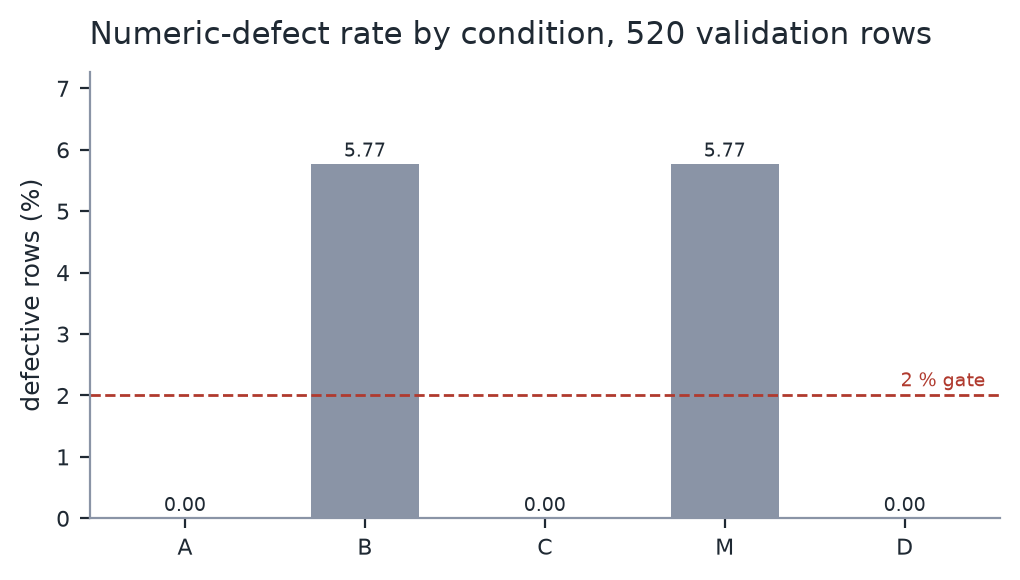
\includegraphics[keepaspectratio]{figures/fig1_cells.png}}
\caption{Numeric-defect rate by condition}
\end{figure}

\begin{longtable}[]{@{}lllllll@{}}
\toprule\noalign{}
cell & numeric & rate & grounding & role & contradiction & anchor \\
\midrule\noalign{}
\endhead
\bottomrule\noalign{}
\endlastfoot
A & \textbf{0} & 0.00 \% & 0 & 0 & 0 & \textbf{520/520} \\
B & 30 & 5.77 \% & 33 & 57 & 0 & 188/520 \\
C & \textbf{0} & 0.00 \% & 1 & 17 & 0 & \textbf{520/520} \\
M & 30 & 5.77 \% & 32 & 43 & 0 & 191/520 \\
D & 0 & 0.00 \% & 0 & 0 & 0 & 262/520 \\
\end{longtable}

McNemar, B against A: 30 vs 0, exact p = 2$\cdot$0.5$^{30}$ $\approx$ 1.9 $\times$ 10$^{-9}$ (the
scorer's stored field reads 0.0, a float underflow, so the value is
derived from the discordant counts). The seams certify: C leaks 0 of B's
numeric values and M leaks 0 of A's. D substitutes A on 114 of 520 rows
(21.9 \%), inside its pre-registered 25 \% ceiling.

Note what the cell table does \emph{not} show: B's numeric rate (5.77
\%) is the highest in the table, but C --- A's numbers inside B's prose
--- is exact. The numbers, not the prose, carry the defect.

\subsubsection{6.2 Confirmatory pass}\label{confirmatory-pass}

\begin{figure}
\centering
\pandocbounded{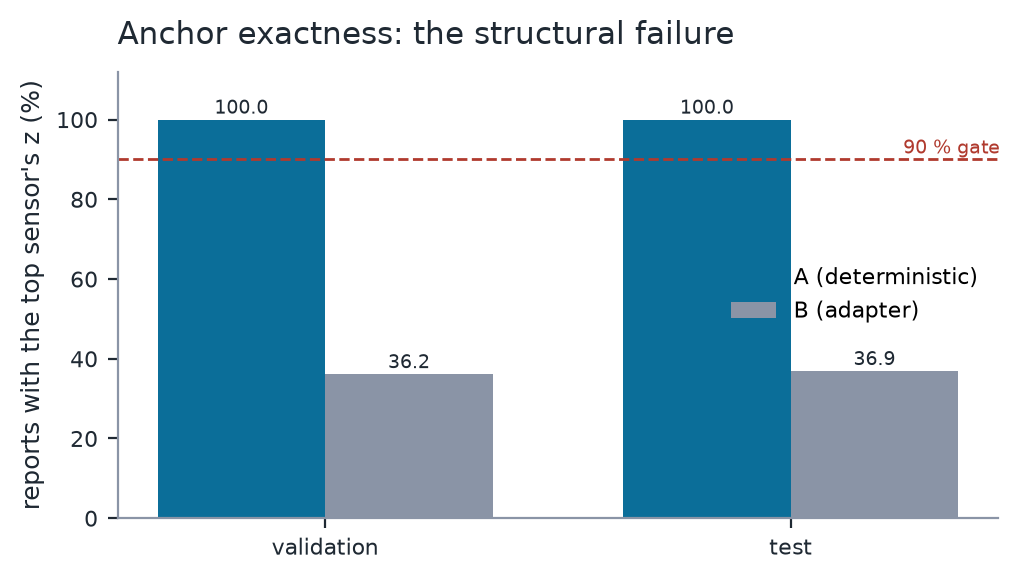
\includegraphics[keepaspectratio]{figures/fig4_anchor.png}}
\caption{Anchor exactness}
\end{figure}

\begin{longtable}[]{@{}
  >{\raggedright\arraybackslash}p{(\linewidth - 8\tabcolsep) * \real{0.2000}}
  >{\raggedright\arraybackslash}p{(\linewidth - 8\tabcolsep) * \real{0.2000}}
  >{\raggedright\arraybackslash}p{(\linewidth - 8\tabcolsep) * \real{0.2000}}
  >{\raggedright\arraybackslash}p{(\linewidth - 8\tabcolsep) * \real{0.2000}}
  >{\raggedright\arraybackslash}p{(\linewidth - 8\tabcolsep) * \real{0.2000}}@{}}
\toprule\noalign{}
\begin{minipage}[b]{\linewidth}\raggedright
check
\end{minipage} & \begin{minipage}[b]{\linewidth}\raggedright
A
\end{minipage} & \begin{minipage}[b]{\linewidth}\raggedright
B
\end{minipage} & \begin{minipage}[b]{\linewidth}\raggedright
gate
\end{minipage} & \begin{minipage}[b]{\linewidth}\raggedright
verdict
\end{minipage} \\
\midrule\noalign{}
\endhead
\bottomrule\noalign{}
\endlastfoot
numeric & \textbf{0 (0.00 \%)} & \textbf{40 (1.26 \%)} & $\leq$ 2 \% & both
pass \\
grounding & 250 (7.89 \%) & 325 (10.26 \%) & $\leq$ 2 \% & both fail \\
contradiction & 0 & 5 (0.16 \%) & $\leq$ 2 \% & both pass \\
instrument role & 0 & 458 (14.46 \%) & $\leq$ 2 \% & B fails \\
anchor exact & \textbf{3,168 (100 \%)} & \textbf{1,170 (36.93 \%)} & $\geq$
90 \% & B fails \\
\end{longtable}

McNemar: 40 vs 0, exact p = 2$\cdot$0.5$^{40}$ $\approx$ 1.8 $\times$ 10$^{-12}$ (stored as 0.0 by
underflow, derived from the counts). B's anchor failures decompose into
an omitted z-score (46.1 \% of rows), a value contradicting the stored
one (6.4 \%), and a named sensor that was never on the page (10.6 \%).

This is the paper's central contrast. The adapter \textbf{meets the
numeric budget on held-out data} --- a genuinely good result for a 2B
model writing technical prose --- and simultaneously \textbf{fails every
structural check}, by margins no reviewer would call marginal.

\subsubsection{6.3 Where the numeric defects actually
are}\label{where-the-numeric-defects-actually-are}

\begin{figure}
\centering
\pandocbounded{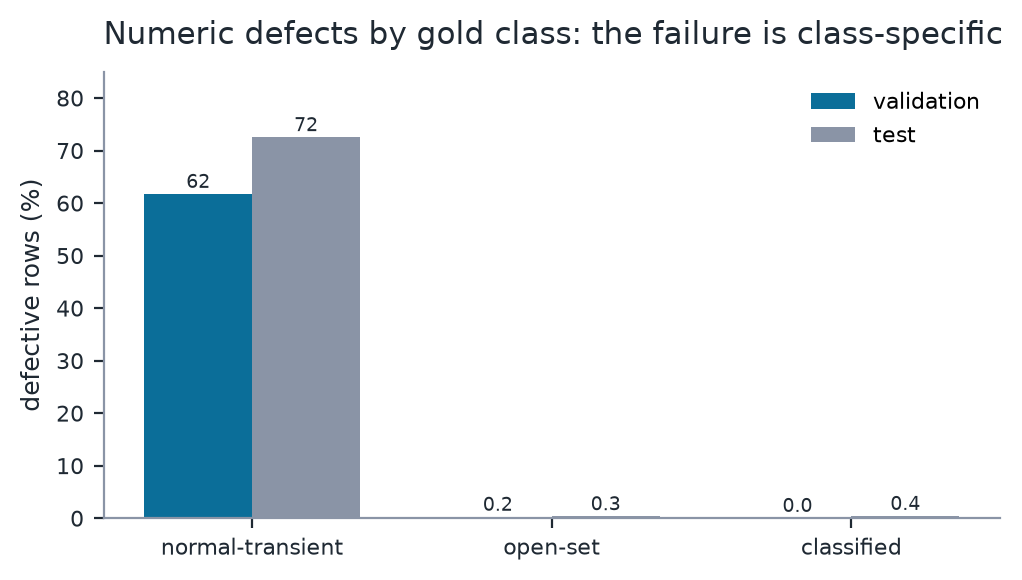
\includegraphics[keepaspectratio]{figures/fig2_stratified.png}}
\caption{Defects by gold class}
\end{figure}

\begin{longtable}[]{@{}lll@{}}
\toprule\noalign{}
gold class & fit set & confirmatory \\
\midrule\noalign{}
\endhead
\bottomrule\noalign{}
\endlastfoot
normal-transient & \textbf{29/47 = 61.7 \%} & \textbf{29/40 = 72.5
\%} \\
open-set & 1/454 = 0.2 \% & 6/1,814 = 0.3 \% \\
classified & 0/19 = 0 \% & 5/1,314 = 0.4 \% \\
\end{longtable}

The unstratified rates (5.77 \% vs 1.26 \%) differ by 4.6$\times$, and the gap
is almost entirely composition: the only class where the writer fails is
9.0 \% of the fit set and 1.3 \% of the confirmatory pass. Within the
failing class the counts are nearly identical (29 and 29). An earlier
draft of this work read the unstratified gap as split dependence;
stratifying dissolves it.

The two splits were rendered from slightly different prompt builds (\S7,
limitation 2), so we claim \textbf{consistency across two builds}, not
stability across identical conditions: in both, the defect concentrates
on no-alarm narratives and is near-absent elsewhere. The matched counts
do not depend on the template difference, and the comparison is within
class throughout.

The failure mode is specific and reproducible: writing a \emph{no-alarm}
narrative, the adapter attaches inequality claims to detectors whose
stored values point the other way. That is an error a deployment can
monitor for directly (count inequality claims in normal-transient
reports), which is more useful than a global defect rate.

\subsubsection{6.4 Diagnosis channel}\label{diagnosis-channel}

\begin{figure}
\centering
\pandocbounded{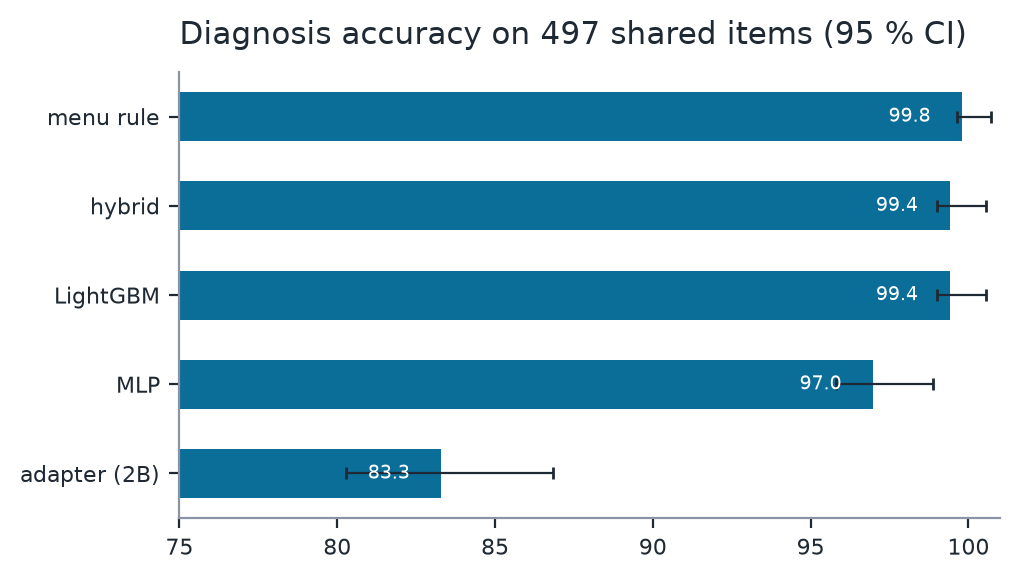
\includegraphics[keepaspectratio]{figures/fig3_classifier.png}}
\caption{Diagnosis accuracy}
\end{figure}

On the 497 items where all systems produce a label:

\begin{longtable}[]{@{}lll@{}}
\toprule\noalign{}
system & accuracy & 95 \% CI \\
\midrule\noalign{}
\endhead
\bottomrule\noalign{}
\endlastfoot
menu rule & 1.0000 & 0.9923--1.0000 \\
hybrid (shipped) & 0.9960 & 0.9854--0.9989 \\
LightGBM & 0.9980 & 0.9887--0.9996 \\
MLP & 0.9799 & 0.9634--0.9890 \\
adapter alone & 0.8330 & 0.7977--0.8632 \\
\end{longtable}

The ``adapter alone'' row is the \textbf{protocolA} adapter at
checkpoint 300 (\texttt{outputs/\allowbreak{}tep\_\allowbreak{}rca\_\allowbreak{}v2\_\allowbreak{}protocolA\_\allowbreak{}seed42}), the
checkpoint the macro-F1 selection chose; it is not the adapter named in
\texttt{configs/\allowbreak{}config.yaml} (\texttt{outputs/\allowbreak{}tep\_\allowbreak{}rca\_\allowbreak{}internvl3\_\allowbreak{}2b}),
which is the deployment artefact and is not scored in this table.

Hybrid against LightGBM: 2 vs 1 discordant (b = 2, c = 1), exact p =
1.0. The knowledge-base layer buys \textbf{no accuracy}, and the adapter
as a classifier is clearly behind. The layer's justification must
therefore be explanatory coverage and dialogue grounding, which we do
not claim to have measured as a preference.

\textbf{Re-measured 2026-11-16, after the feature-vocabulary fix.} The
classifier's columns named the manipulated variables \texttt{XMV\_1..11}
while the evidence page prints \texttt{XMV\_42..52}, so 22.4 \% of the
sensors listed on stored pages had no column and contributed nothing.
With the vocabulary aligned and every classifier-side model retrained,
the table above replaces the earlier menu rule 0.9980, hybrid 0.9940,
LightGBM 0.9940 and MLP 0.9698. The adapter row is unchanged: its
predictions never depended on those features. On the cross-fitted
evaluation the same fix moves observable accuracy from 0.9781 to 0.9878
and macro-F1 from 0.9708 to 0.9843, so the paper's diagnosis numbers are
the post-fix ones; the superseded values are kept in the audit record.

\subsubsection{6.5 Preference}\label{preference}

360 pairs, two readers, $\kappa$ = 0.5776 (observed agreement 0.7778, expected
0.4739). Below the declared 0.60 floor, so the preference tier is
reported descriptively and supports no claim. Publishing a preference
\emph{ordering} at this reliability would be the exact error that
judge-noise work warns about \citep{zheng2023judging}.

\subsubsection{6.6 Selection}\label{selection}

A six-rung selector applies pre-registered rungs in order. Rung 1 vetoes
B (5.77 \% against a 1.00 \% ceiling set as A + 1 pp). Rungs 2--4 are
unavailable: preference is below its floor, and no eligible passer
carries an independently verified mechanism claim. Rung 5 compares time
per 520-row pass on a pre-signed cost basis; A and D tie, and the
declared tie-break selects A. The resulting receipt
(\texttt{decided\_by\_rung\ 5}, chosen A, no dollar figure claimed) is
committed with the paper.

D is a legitimate engineering option and it does not lose on any
measured axis --- it simply contributes nothing of its own on the 21.9
\% of rows where it substitutes.

\subsection{7. Limitations}\label{limitations}

\begin{enumerate}
\def\labelenumi{\arabic{enumi}.}
\tightlist
\item
  \textbf{One adapter configuration.} Seed 42, one order on the
  confirmatory pass, greedy decoding. Batch size is a measurement
  parameter, not a neutral setting: only 1 of 12 texts was identical
  between batch 16 and batch 8.
\item
  \textbf{Template drift between splits.} The stored fit-set prompts
  were generated under an earlier prompt build (0 of 520 match the
  current builder byte-for-byte). All cross-split comparisons in this
  paper are therefore within-class, and \S6.3 is the only cross-split
  claim we make.
\item
  \textbf{Instrument history.} The numeric check was revised twice after
  artefacts were found. All numbers here come from the final version;
  the changelog in \S8 records what moved and why, and the superseded
  table is retained.
\item
  \textbf{Ceiling decision.} D's substitution rate is inside its 25 \%
  ceiling on the corrected instrument (21.9 \%), while the signed
  decision predates the correction. We therefore describe D
  conservatively as A with extra steps rather than claim a certified
  pass.
\item
  \textbf{Not measured.} Detector frontier (Table 7), follow-up dialogue
  condition (T), cross-path parity of the two scoring implementations,
  and any latency claim other than the generator's. Each is listed as
  future work rather than estimated.
\item
  \textbf{Figures rebuilt 2026-11-16.} \texttt{fig3}, \texttt{fig6},
  \texttt{fig8} and \texttt{approach\_data.json} were regenerated from
  the retrained artefacts; \texttt{fig7} is unchanged because recall and
  missed abstention did not move. \texttt{fig8} now reads
  \texttt{vocabfix/\allowbreak{}surrogate\_\allowbreak{}wide.json} directly (13 faults retrained),
  so figure and table share one source and no longer disagree with the
  text. Cross-fitted intervals are quoted: accuracy 0.9878
  (0.9783--0.9962), macro-F1 0.9843 (0.9711--0.9947), a cluster
  bootstrap over 497 events.
\end{enumerate}

\subsection{8. Reproducibility and instrument
changelog}\label{reproducibility-and-instrument-changelog}

Every artefact is listed with its SHA-256 and rebuild command in the
release manifest. Figures are rendered from stored JSON by one script,
so a changed number changes the figure. The number sources themselves
are committed under \texttt{docs/\allowbreak{}reports/\allowbreak{}evidence/\allowbreak{}} with SHA-256 hashes
and a claim $\rightarrow$ file index, because the working artefacts live in an
untracked \texttt{outputs/\allowbreak{}} tree;
\texttt{scripts/\allowbreak{}bundle\_\allowbreak{}evidence.py\ -\/\allowbreak{}-check} re-verifies them.

\begin{longtable}[]{@{}
  >{\raggedright\arraybackslash}p{(\linewidth - 10\tabcolsep) * \real{0.1667}}
  >{\raggedright\arraybackslash}p{(\linewidth - 10\tabcolsep) * \real{0.1667}}
  >{\raggedright\arraybackslash}p{(\linewidth - 10\tabcolsep) * \real{0.1667}}
  >{\raggedright\arraybackslash}p{(\linewidth - 10\tabcolsep) * \real{0.1667}}
  >{\raggedright\arraybackslash}p{(\linewidth - 10\tabcolsep) * \real{0.1667}}
  >{\raggedright\arraybackslash}p{(\linewidth - 10\tabcolsep) * \real{0.1667}}@{}}
\toprule\noalign{}
\begin{minipage}[b]{\linewidth}\raggedright
version
\end{minipage} & \begin{minipage}[b]{\linewidth}\raggedright
rule added
\end{minipage} & \begin{minipage}[b]{\linewidth}\raggedright
A (fit)
\end{minipage} & \begin{minipage}[b]{\linewidth}\raggedright
B (fit)
\end{minipage} & \begin{minipage}[b]{\linewidth}\raggedright
A (test)
\end{minipage} & \begin{minipage}[b]{\linewidth}\raggedright
B (test)
\end{minipage} \\
\midrule\noalign{}
\endhead
\bottomrule\noalign{}
\endlastfoot
v1 & numbers attributed to first detector only & 19/520 & 62/520 & 619 &
115 \\
v2 & role matching (\texttt{z=} against stored z) & 13/520 & 50/520 &
619 & 111 \\
\textbf{v3} & identifiers masked & \textbf{0/520} & \textbf{30/520} &
\textbf{0} & \textbf{40} \\
\end{longtable}

The v1$\rightarrow$v3 movement for A (19 $\rightarrow$ 0) is the reason we keep the changelog: a
reader who sees only v3 has no way to know whether zero is a real
property or a lenient check. The reproduction argument is stronger than
the changelog alone --- rebuilding A on the fit set with the v3 checker
yields 0/520, which is what a writer copying from the page must yield.

\subsection{9. Conclusion}\label{conclusion}

A 2B adapter can write industrial fault reports that stay inside a
numeric-fidelity budget on held-out data, and it will still fail the
checks that decide whether an operator can trust a paragraph: it will
drop the top sensor's z-score, call a detector an actuator, and mention
a tag that was never on the page. The failures are concentrated,
monitorable and class-specific rather than diffuse. Keep the diagnosis
deterministic, measure structure as carefully as you measure numbers,
and report stratified rates --- an unstratified rate hid both the size
and the shape of the adapter's defect for several revisions of this
work.

\begin{center}\rule{0.5\linewidth}{0.5pt}\end{center}

\subsubsection{Figure list}\label{figure-list}

\begin{longtable}[]{@{}
  >{\raggedright\arraybackslash}p{(\linewidth - 4\tabcolsep) * \real{0.3333}}
  >{\raggedright\arraybackslash}p{(\linewidth - 4\tabcolsep) * \real{0.3333}}
  >{\raggedright\arraybackslash}p{(\linewidth - 4\tabcolsep) * \real{0.3333}}@{}}
\toprule\noalign{}
\begin{minipage}[b]{\linewidth}\raggedright
file
\end{minipage} & \begin{minipage}[b]{\linewidth}\raggedright
content
\end{minipage} & \begin{minipage}[b]{\linewidth}\raggedright
data source
\end{minipage} \\
\midrule\noalign{}
\endhead
\bottomrule\noalign{}
\endlastfoot
\texttt{figures/\allowbreak{}fig1\_\allowbreak{}cells.png} & numeric rate by condition with the 2
\% gate & \texttt{n4\_cells.json} \\
\texttt{figures/\allowbreak{}fig2\_\allowbreak{}stratified.png} & defects by gold class, both
splits & recomputed with \texttt{measure} \\
\texttt{figures/\allowbreak{}fig3\_\allowbreak{}classifier.png} & diagnosis accuracy with 95 \%
CIs & \texttt{classifier\_contrasts.json} \\
\texttt{figures/\allowbreak{}fig4\_\allowbreak{}anchor.png} & anchor exactness against the 90 \%
gate & \texttt{n4\_cells.json}, \texttt{test\_contrast.json} \\
\end{longtable}

\subsubsection{Non-claims}\label{non-claims}

No claim that the adapter is more faithful than the deterministic
writer; no cross-split rate comparison; no preference ordering; no
mechanism-quality claim; no latency claim outside the generator; no
detector-frontier comparison.

\bibliography{references.bib}

\end{document}
